\documentclass[10pt,a4paper]{article}

\usepackage[utf8]{inputenc}
\usepackage[T1]{fontenc}
\usepackage{lmodern}
\usepackage{amsmath, amssymb, mathtools}
\usepackage{amsthm}
\usepackage{graphicx}
\usepackage{booktabs}
\usepackage[labelfont=bf,textfont=it]{caption}
\usepackage{subcaption}
\usepackage[left=2cm,right=2.7cm,top=2.1cm,bottom=2.5cm,includeheadfoot]{geometry}
\usepackage{setspace}
\usepackage[english]{babel}
\usepackage{xcolor}
\usepackage{hyperref}
\hypersetup{colorlinks=true, linkcolor={blue!50!black},
            citecolor={blue!50!black}, urlcolor={blue!50!black}}
\DeclareMathOperator*{\argmin}{arg\,min}

% - Theorem boxes, same style as the thesis -
\usepackage[most]{tcolorbox}
\usetikzlibrary{positioning}
\tcbuselibrary{theorems, breakable, skins}
\tcbset{
  mythmstyle/.style={
    enhanced, sharp corners, boxrule=0.8pt,
    colback=white, colframe=black!75, coltitle=black,
    fonttitle=\bfseries,
    left=8pt, right=8pt, top=8pt, bottom=8pt,
    attach boxed title to top left={yshift=-2mm, xshift=4mm},
    boxed title style={colback=black!8, colframe=black!75,
      sharp corners, boxrule=0.8pt},
    before skip=10pt, after skip=10pt
  }
}
\newtcbtheorem[number within=section]{theorem}{Theorem}%
{mythmstyle,colback=blue!2!white,colframe=blue!50!black,colbacktitle=blue!10!white}{th}
\newtcbtheorem[use counter from=theorem]{definition}{Definition}%
{mythmstyle,breakable,colback=orange!3!white,colframe=orange!70!black,colbacktitle=orange!15!white}{def}

% numbers of examples.ipynb,
% written 2026-07-12, verified against the re-run of 2026-07-29/30
\newcommand{\drYzero}{57.042}
\newcommand{\drRelErr}{0.45}
\newcommand{\hjbRef}{4.5903}
\newcommand{\hjbRelErr}{0.01}
\newcommand{\hjbLamMaxDev}{1.20}
\newcommand{\acYzero}{0.0528}
\newcommand{\acRelErr}{0.02}


\title{Documentation \\
\emph{Testing Examples of the Deep BSDE Solver}}
\author{Patrick Streeb}
\date{\today}

\begin{document}
\onehalfspacing
\maketitle
\tableofcontents

\section{Introduction}
\label{sec:summary}
Grid-based numerical methods for partial differential equations have a computational cost that grows exponentially with the dimension $d$, which is known as the curse of dimensionality. Nevertheless, many practical applications lead to high-dimensional problems. Monte Carlo methods applied to stochastic representations of PDE solutions work well in many cases, but perform less effectively when nested Monte Carlo simulation is required, since the computational cost does not scale linearly with the dimension of the problem. A second approach is the deep BSDE method of Han, Jentzen, and E \cite{Han2018}, which indeed overcomes the curse of dimensionality. By reformulating a large class of PDEs as backward stochastic differential equations (BSDEs) and discretizing these equations, the resulting recursion contains two unknowns. Time-dependent neural networks are therefore used to approximate one of them. Increasing the dimension of the state only adds further components to the recursion, which can be evaluated in parallel. The article by Han, Jentzen, and E \cite{Han2018} is our main reference, and we refer to it as the reference paper or, for short, the paper. \\ \
\begin{figure}[htb]
\centering
\resizebox{\linewidth}{!}{%
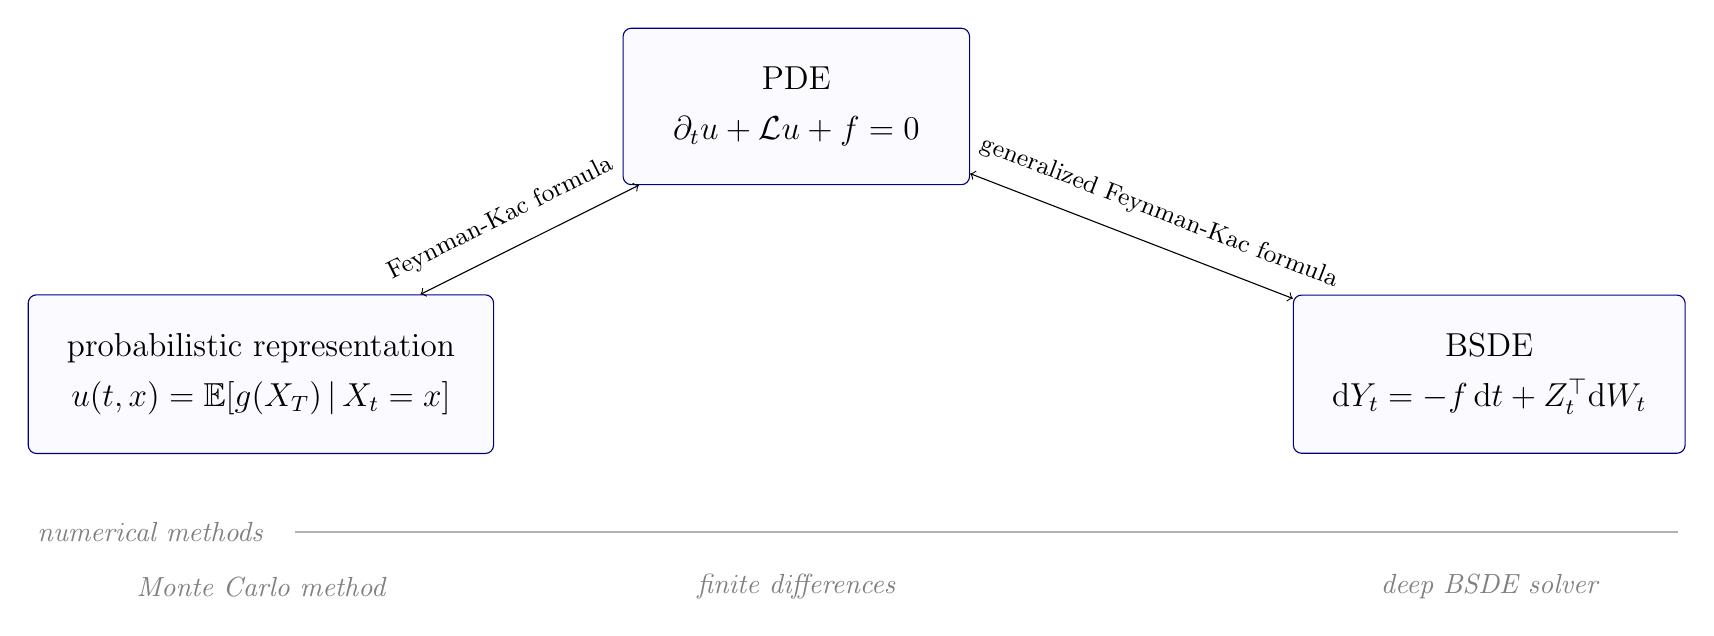
\begin{tikzpicture}[
  box/.style={draw=blue!50!black, fill=blue!2!white, rounded corners=3pt,
    align=center, inner sep=14pt, minimum height=1.8cm, minimum width=4.4cm,
    font=\large},
  meth/.style={font=\itshape, text=black!50, align=center},
  thlab/.style={above=4pt, sloped, font=\small}]
\node[box] (prob) at (0,0)
  {probabilistic representation\\[4pt]$u(t,x) = \mathbb E\!\left[g(X_T)\,\middle|\,X_t = x\right]$};
\node[box] (pde) at (6.8,3.4)
  {PDE\\[4pt]$\partial_t u + \mathcal L u + f = 0$};
\node[box] (bsde) at (15.6,0)
  {BSDE\\[4pt]$\mathrm dY_t = -f\,\mathrm dt + Z_t^{\top}\mathrm dW_t$};
\draw[<->] (prob) -- (pde)
  node[thlab, pos=0.43] {Feynman-Kac formula};
\draw[<->] (pde) -- (bsde)
  node[thlab, pos=0.55] {generalized Feynman-Kac formula};

\node[meth, anchor=west] (nm) at (prob.west |- 0,-2.0) {numerical methods};
\draw[gray!60, thick] ([xshift=8pt]nm.east) -- (18.0,-2.0);
\node[meth] at (0,-2.7) {Monte Carlo method};
\node[meth] at (6.8,-2.7) {finite differences};
\node[meth] at (15.6,-2.7) {deep BSDE solver};
\end{tikzpicture}}
\caption{The three formulations of a parabolic terminal value problem
and their numerical methods.}
\label{fig:route}
\end{figure}
\newline
The goal of this documentation is to reproduce the examples in the paper, where the approach was introduced first. To try out our own architectures, we adapted the solver architecture to our own version. We could sometimes yield better results, than the ones postulated in the paper. Overall, the results are reproducible and we can confirm them for the presented examples. All source code developed for this project is available in the accompanying GitHub repository.\footnote{\url{https://github.com/patrickstreeb/deep-bsde-solver-examples}} In total, there were four examples investigated.
\begin{itemize}
    \item [(1)] For the Hamilton-Jacobi-Bellman equation of
a linear-quadratic control problem the trained value matches the Monte
Carlo reference with a relative error of \hjbRelErr\,\% (paper
$0.17\,\%$).
\item [(2)] For the Allen-Cahn equation the error against the
branching-diffusion value is \acRelErr\,\% (paper $0.30\,\%$). 
\item [(3)] For the
nonlinear Black-Scholes equation with default risk the error against the
multilevel Picard value is \drRelErr\,\% (paper $0.46\,\%$). 
\item [(4)] The final example was a
reaction-diffusion equation, where we showed, that the accuracy improves with the number of hidden layers per subnetwork. With the 40000 epochs of the paper the error drops to $0.93\,\%$ at four hidden layers, against $0.53\,\%$ in the paper.
\end{itemize}



\section{Preliminaries}
\label{sec:preliminaries}

We fix a finite horizon $T\in(0,\infty)$ and a filtered probability
space \((\Omega,\mathcal F,\mathbb P)\) with filtration $(\mathcal F_t)_{t\in[0,T]}$ satisfying the usual conditions and carrying a $d$-dimensional standard Brownian motion $W=(W_t)_{t\in[0,T]}$. Every expectation in this documentation refers to this space, we write $\mathbb E$ for $\mathbb E^{\mathbb P}$ and $\mathbb E[\,\cdot\mid\mathcal F_t]$ for the conditional expectation given $\mathcal F_t$. Let
\[
\mu\colon[0,T]\times\mathbb R^d\to\mathbb R^d,
\qquad
\sigma\colon[0,T]\times\mathbb R^d\to\mathbb R^{d\times d}
\]
be measurable. Suppose that there exists a constant $L>0$ such that, for all $t\in[0,T]$ and $x,y\in\mathbb R^d$,
\begin{align*}
\lvert\mu(t,x)-\mu(t,y)\rvert
+\lVert\sigma(t,x)-\sigma(t,y)\rVert
&\leq L\lvert x-y\rvert \\
\lvert\mu(t,x)\rvert+\lVert\sigma(t,x)\rVert
&\leq L(1+\lvert x\rvert).
\end{align*}
Here, $\lVert\cdot\rVert$ denotes the Frobenius norm and $I_d\in\mathbb R^{d\times d}$ the $d$-dimensional identity matrix. For each
$(t,x)\in[0,T]\times\mathbb R^d$, let
$X^{t,x}=(X_s^{t,x})_{s\in[t,T]}$ denote the unique strong solution of
\begin{equation*}
X_s^{t,x}
=
x+\int_t^s\mu(r,X_r^{t,x})\,\mathrm dr
+\int_t^s\sigma(r,X_r^{t,x})\,\mathrm dW_r,
\qquad s\in[t,T].
\end{equation*}
The stochastic integral is understood in the It\^o sense. The classical Feynman--Kac formula represents solutions of linear parabolic terminal value problems as expectations; see \cite[Chapter~8]{Oksendal2003}. We denote by
$\mathcal H_xu=(\partial_{x_i x_j}u)_{i,j=1}^d$ the Hessian of $u$ with
respect to the spatial variable.
\begin{theorem}[breakable]{Feynman--Kac Formula}{feynman-kac}
Let $g\colon\mathbb R^d\to\mathbb R$ be continuous, and let \(u\in C([0,T]\times\mathbb R^d)
   \cap C^{1,2}([0,T)\times\mathbb R^d)\) satisfy
\begin{align*}
\partial_tu(t,x)
+\frac12\operatorname{Tr}\!\left(
  \sigma\sigma^\top(t,x)\mathcal H_xu(t,x)
 \right)
+\mu(t,x)\cdot\nabla_xu(t,x)
&=0 \\
u(T,x)&=g(x) 
\end{align*}
for $ (t,x)\in[0,T)\times\mathbb R^d.$ Assume that there exists a constant $C>0$ such that
\[
\lvert u(t,x)\rvert
+\left\lvert
  \sigma^\top(t,x)\nabla_xu(t,x)
 \right\rvert
\leq C(1+\lvert x\rvert)
\]
for every $(t,x)\in[0,T)\times\mathbb R^d$. Then
\[
u(t,x)
=
\mathbb E
\left[g\!\left(X_T^{t,x}\right)\right],
\qquad (t,x)\in[0,T]\times\mathbb R^d.
\]
\end{theorem}
\begin{proof}
    See \cite[Chapter~8]{Oksendal2003}.
\end{proof}
If we for example take $d=1$, $\mu=0$, $\sigma=1$, and $g(x)=x^2$ we get
\[
X_s^{t,x}=x+W_s-W_t,
\qquad s\in[t,T],
\]
and therefore
\[
X_T^{t,x}=x+W_T-W_t.
\]
We can now apply the Theorem of Feynman and Kac. Since $W$ is a Brownian motion, we have $W_T-W_t\sim\mathcal N(0,T-t)$ by definition and since it lives on $(\Omega, \mathcal{F,} \mathbb{P})$, the expectation of the increment under $\mathbb{P}$ is zero and the squared increment is equal to $T-t$. We get
\begin{align*}
u(t,x)
&=\mathbb E\!\left[g\!\left(X_T^{t,x}\right)\right] \\
&=\mathbb E\!\left[(x+W_T-W_t)^2\right] \\
&=x^2
  +2x\,\mathbb E[W_T-W_t]
  +\mathbb E\!\left[(W_T-W_t)^2\right] \\
&=x^2+T-t.
\end{align*}
The generalization to semilinear equations replaces the conditional expectation by a pair of processes solving a backward stochastic differential equation. We first fix the class of equations.
\begin{definition}{Semilinear Parabolic Terminal Value Problem}{semilinear-pde}
Let $f\colon[0,T]\times\mathbb R^d\times\mathbb R\times\mathbb R^d
\to\mathbb R$ and $g\colon\mathbb R^d\to\mathbb R$ be measurable. A
\emph{semilinear parabolic terminal value problem} is the problem of
finding $u\in C^{1,2}([0,T]\times\mathbb R^d)$ with
\begin{align*}
\partial_t u(t,x)
+ \tfrac12 \operatorname{Tr}\!\left(\sigma\sigma^{\top}(t,x)\,
  \mathcal{H}_x\, u(t,x)\right) & \\
+ \nabla u(t,x)\cdot\mu(t,x)
+ f\!\left(t,x,u(t,x),\sigma^{\top}(t,x)\nabla u(t,x)\right) &= 0,\\
u(T,x) &= g(x).
\end{align*}
We call $\mu$ the drift, $\sigma$ the diffusion coefficient or volatility, $f$ the generator or driver and $g$ the terminal condition. The involved PDE is called \textit{semilinear parabolic} PDE.
\end{definition}
The equation is parabolic through the second order diffusion part, and semilinear because the highest order derivatives enter linearly while $u$ and $\nabla u$ may enter nonlinearly through $f$. For example, the Allen-Cahn equation of Section~\ref{sec:ac},
\[
\partial_t u(t,x) = \Delta u(t,x) + u(t,x) - u(t,x)^3,
\]
is a semilinear parabolic PDE. We calculate, for $\sigma = \sqrt{2}\,I_d$,
\begin{align*}
\tfrac12\operatorname{Tr}\!\left(\sigma\sigma^{\top}\,
\mathcal{H}_x\, u\right)
&= \tfrac12\operatorname{Tr}\!\left(2\,I_d\,
\mathcal{H}_x\, u\right)
= \sum_{i=1}^{d}\frac{\partial^2 u}{\partial x_i^2}
= \Delta u,
\end{align*} 
and choose the parameters
\begin{equation*}
\mu = 0,
\qquad
\sigma = \sqrt{2}\,I_d,
\qquad
f(t,x,y,z) = y - y^3.
\end{equation*}


A\textit{ backward stochastic differential equation} (BSDE) can be described by a terminal random variable $\xi$ and a generator $f$ such that a solution is a pair of adapted processes $(Y_t, Z_t)_{t\in[0,T]}$ satisfying
\[
Y_t = \xi + \int_t^T f(s,Y_s,Z_s)\,\mathrm ds
- \int_t^T Z_s^{\top}\,\mathrm dW_s.
\]
Existence and uniqueness of this pair, together with the connection to partial differential equations, go back to \cite{PardouxPeng1990}.
\section{The Deep BSDE Method}
\label{sec:method}
We want to compute the value $u(0,\xi)$ of the solution of a semilinear
parabolic terminal value problem (Definition~\ref{def:semilinear-pde}) in
high dimension $d$. The main idea is to introduce a system consisting of a forward and a backward stochastic differential equation
\begin{align*}
X_t
&= \xi+\int_0^t\mu(s,X_s)\,\mathrm ds
+\int_0^t\sigma(s,X_s)\,\mathrm dW_s, \\
Y_t
&= g(X_T)+\int_t^T f(s,X_s,Y_s,Z_s)\,\mathrm ds
-\int_t^T Z_s^\top\,\mathrm dW_s.
\end{align*}
In differential notation, this system becomes
\begin{align}
\mathrm dX_t
&=\mu(t,X_t)\,\mathrm dt+\sigma(t,X_t)\,\mathrm dW_t,
& X_0&=\xi, \nonumber\\
\mathrm dY_t
&=-f(t,X_t,Y_t,Z_t)\,\mathrm dt+Z_t^\top\,\mathrm dW_t,
& Y_T&=g(X_T).
\label{eq:fbsde}
\end{align}
The following theorem draws the connection with the corresponding
PDE.
\begin{theorem}[breakable]{Generalized Feynman--Kac Formula}{feynman-kac-general}
Let $f$ be globally Lipschitz continuous in $(x,y,z)$ and let $g$ be
globally Lipschitz continuous. Suppose that both functions have at most
linear growth. Let
\[
u\in C([0,T]\times\mathbb R^d)
\cap C^{1,2}([0,T)\times\mathbb R^d)
\]
solve the problem in Definition~\ref{def:semilinear-pde}. Assume, in
addition, that $u$ and $\sigma^\top\nabla_xu$ have at most linear growth in the spatial variable. Then
\begin{equation}
Y_t:=u(t,X_t),
\qquad
Z_t:=\sigma^\top(t,X_t)\nabla_xu(t,X_t),
\qquad t\in[0,T],
\label{eq:genfeynman}
\end{equation}
form the unique solution of the backward equation in \eqref{eq:fbsde}.
\end{theorem}

\begin{proof}
See \cite{ElKarouiPengQuenez1997}.
\end{proof}
Consequently, instead of solving the PDE directly, we may solve the
corresponding forward--backward stochastic differential equation
(FBSDE). Solving \eqref{eq:fbsde} forward in time requires the initial values $Y_0$ and $Z_0$, which are the unknown. On a grid $0=t_0<t_1<\dots<t_N=T$ with $\Delta t_n = t_{n+1}-t_n$ and $\Delta W_n = W_{t_{n+1}}-W_{t_n}$ we discretize \eqref{eq:fbsde} by the Euler scheme
\begin{align}
X_{t_{n+1}} &= X_{t_n} + \mu(t_n,X_{t_n})\,\Delta t_n
+ \sigma(t_n,X_{t_n})\,\Delta W_n, \nonumber\\
Y_{t_{n+1}} &= Y_{t_n} - f\!\left(t_n,X_{t_n},Y_{t_n},Z_{t_n}\right)
\Delta t_n + Z_{t_n}^{\top}\Delta W_n,
\qquad n = 0,\dots,N-1.
\label{eq:euler}
\end{align}
We make \eqref{eq:euler} computable by three substitutions. The unknown initial value $Y_{t_0}$ becomes a trainable parameter $\theta_{u_0}\in\mathbb R$, the unknown initial gradient $Z_{t_0}$ becomes a trainable parameter $\theta_{\nabla u_0}\in\mathbb R^d$, and the process $Z$ is approximated on the grid by feedforward neural networks $\varphi^{\theta_n}\colon\mathbb R^d\to\mathbb R^d$ with parameters $\theta_n$. The scheme becomes
\begin{align}
X_{t_{n+1}} &= X_{t_n} + \mu(t_n,X_{t_n})\,\Delta t_n
+ \sigma(t_n,X_{t_n})\,\Delta W_n, \nonumber\\
Y^{\theta}_{t_{n+1}} &= Y^{\theta}_{t_n}
- f\!\left(t_n,X_{t_n},Y^{\theta}_{t_n},Z^{\theta}_{t_n}\right)\Delta t_n
+ \left(Z^{\theta}_{t_n}\right)^{\top}\Delta W_n,
\label{eq:euler-nn}
\end{align}
with
\begin{equation}
Y^{\theta}_{t_0} = \theta_{u_0},
\qquad
Z^{\theta}_{t_0} = \theta_{\nabla u_0},
\qquad
Z^{\theta}_{t_n} = \varphi^{\theta_n}(X_{t_n}),
\quad n = 1,\dots,N-1,
\end{equation}
and the full parameter vector is
\begin{equation}
\theta = \left(\theta_{u_0},\theta_{\nabla u_0},
\theta_1,\dots,\theta_{N-1}\right).
\end{equation}
The terminal value $Y^{\theta}_{t_N}$ of \eqref{eq:euler-nn} is an estimate of $g(X_{t_N})$, and we train all parameters jointly on the expected terminal loss
\begin{equation*}
\ell(\theta)
= \mathbb E\left[\left|g(X_{t_N}) - Y^{\theta}_{t_N}\right|^2\right].
\end{equation*}
The expectation is taken with respect to the underlying probability
measure $\mathbb P$, that is, over the Brownian sample paths. In practice,
we replace it by the empirical average over $M$ independent simulated
trajectories. The deep BSDE estimator of the solution value at the point $(0,\xi)$ is the trained initial parameter,
\begin{equation}
\hat u_{\mathrm{NN}}(0,\xi) := \theta_{u_0}^{\ast},
\qquad
\theta^{\ast} \in \argmin_{\theta}\;
\frac1M \sum_{m=1}^{M}
\left|g\big(X_{t_N}^{(m)}\big) - Y^{\theta,(m)}_{t_N}\right|^2,
\label{eq:nn-estimator}
\end{equation}
where $M$ is the number of simulated paths. All numerical results below
compare $\hat u_{\mathrm{NN}}(0,\xi)$ with reference values for $u(0,\xi)$.

\section{Implementation}
\label{sec:setup}
We use our own implementation of the deep BSDE solver inspired by the author's implementation \cite{DeepBSDErepo}, but allow to test for different network structures. For each $n=1,\dots,N-1$, the network $\varphi^{\theta_n}$ has $H$ hidden layers. Setting
\[
h_n^0:=X_{t_n},
\]
the output of its $\ell$-th hidden layer is defined recursively by
\begin{equation*}
h_n^\ell
:=
\rho\!\left(A_n^\ell h_n^{\ell-1}+b_n^\ell\right),
\qquad \ell=1,\dots,H,
\end{equation*}
where $A_n^\ell$ and $b_n^\ell$ denote the weight matrix and bias vector of the $\ell$-th layer, respectively, and $\rho$ is an activation function applied componentwise. The output layer is given by
\begin{equation*}
\varphi^{\theta_n}(X_{t_n})
:=
A_n^{H+1}h_n^H+b_n^{H+1},
\end{equation*}
where
\[
\theta_n
:=
\left((A_n^\ell,b_n^\ell)\right)_{\ell=1}^{H+1}
\]
collects all trainable parameters of the network. Consequently,
\[
Z_{t_n}^\theta
=
\varphi^{\theta_n}(X_{t_n}),
\qquad n=1,\dots,N-1.
\]
\begin{figure}[htb]
\centering
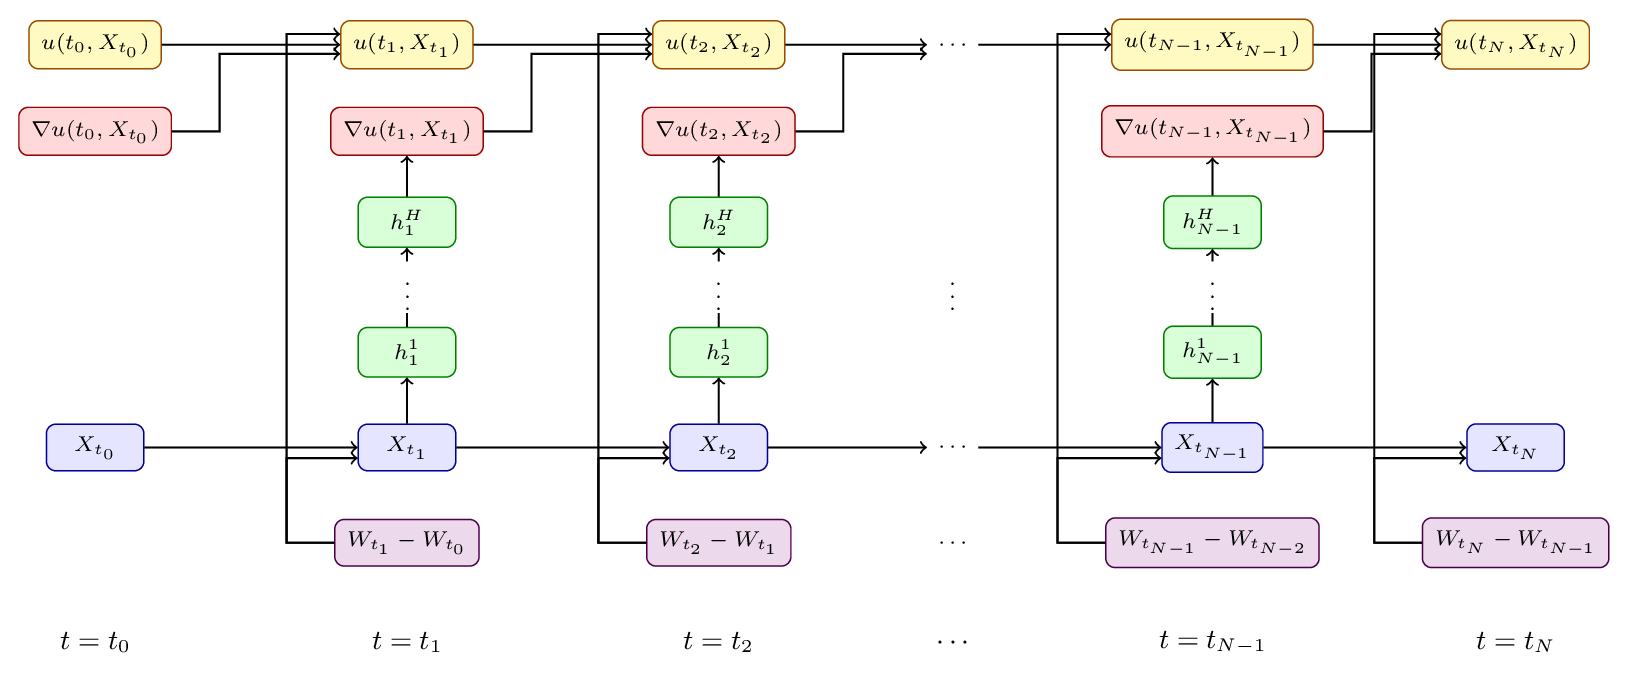
\includegraphics[width=\linewidth]{figures/deep_bsde_network.png}
\caption{Unrolled architecture of the deep BSDE solver, one column per
time step, illustration after \cite{Han2018}.}
\label{fig:solver}
\end{figure}

Furthermore we aim to apply the code to financial problems in later works. Each equation enters as a PDE object holding the coefficients of Definition~\ref{def:semilinear-pde}, the drift, the diffusion, the generator and the terminal condition. The network we used for results in this documentation consists of subnetworks $\varphi^{\theta_n}$ and has one $d$-dimensional input layer, two hidden layers of width $110$ with $\tanh$ activation and no batch normalization, and a $d$-dimensional linear output layer. We optimize with Adam under a decaying learning rate. The initial value $\theta_{u_0}$ starts at a problem-specific guess, according to the initialization range of the paper. From there we iterate forward, taking into account the neural network approximations of $Z$, generated diffusion $X$ and Brownian motion increments $\mathrm dW_t$ in each timestep, see Figure~\ref{fig:solver}.

The used parameters are given in the Tables~\ref{tab:hjb-params}, \ref{tab:ac-params}, \ref{tab:dr-params} and~\ref{tab:rd-params}. The notebook \texttt{examples.ipynb} guides through the setup and produces all results presented in this documentation.

\section{Examples}
\label{sec:examples}
In this Section we study the examples presented in the main article \cite{Han2018}.
\subsection{Hamilton-Jacobi-Bellman Equation}
\label{sec:hjb}
Given is the stochastic control problem
\begin{align*}
\inf_{\{m_t\}_{t\in[0,T]}}\;
& \mathbb E\left[\int_0^T \lVert m_t\rVert^2\,\mathrm dt
+ g(X_T)\right], \\
\mathrm dX_t
&= 2\sqrt{\lambda}\, m_t\,\mathrm dt + \sqrt{2}\,\mathrm dW_t,
\qquad X_0 = x,
\end{align*}
where $\lambda>0$, \(X=(X_t)_{t\in[0,T]}\) and \(m=(m_t)_{t\in[0,T]}\) are \(\mathbb{R}^{100}\)-valued processes, and \(W=(W_t)_{t\in[0,T]}\) is a \(100\)-dimensional Brownian motion. The terminal condition is
\begin{equation*}
g(x) = \ln\!\left(\tfrac12\left(1+\lVert x\rVert^2\right)\right).
\end{equation*}
One can show, that the value function
$$u(t,x) := \inf_{\{m_t\}_{t\in[0,T]}}\; \mathbb E\left[\int_t^T \lVert m_s\rVert^2\mathrm ds + g(X_T)\Big| X_t = x\right]$$
is the solution of the Hamilton-Jacobi-Bellman equation
\begin{equation}
\partial_t u(t,x) + \Delta u(t,x)
+ \min_{m\in\mathbb R^{100}}
\left(2\sqrt{\lambda}\, m\cdot\nabla u(t,x) + \lVert m\rVert^2\right) = 0,
\qquad
u(T,x) = g(x).
\label{eq:hjb-min}
\end{equation}
To evaluate the minimum in \eqref{eq:hjb-min} we introduce, for fixed $(t,x)$, the function
\begin{equation}
F(m) := 2\sqrt{\lambda}\, m\cdot\nabla u(t,x) + \lVert m\rVert^2,
\qquad m\in\mathbb R^{100},
\label{eq:hjb-F}
\end{equation}
and compute
\begin{align*}
\nabla F(m) &= 2\sqrt{\lambda}\,\nabla u(t,x) + 2m,
\\
\mathcal{H}\, F(m) &= 2\,I_d.
\end{align*}
The Hessian is positive definite, so $F$ is strictly convex and its unique stationary point is the global minimum. We solve the first order condition and insert the minimizer into \eqref{eq:hjb-F},
\begin{align}
0 &= \nabla F(m^{\ast})
= 2\sqrt{\lambda}\,\nabla u(t,x) + 2m^{\ast},
\nonumber\\
m^{\ast} &= -\sqrt{\lambda}\,\nabla u(t,x),
\nonumber\\
F(m^{\ast})
&= -2\lambda\,\lVert\nabla u(t,x)\rVert^2
+ \lambda\,\lVert\nabla u(t,x)\rVert^2
= -\lambda\,\lVert\nabla u(t,x)\rVert^2 .
\label{eq:hjb-minimizer}
\end{align}
Inserting \eqref{eq:hjb-minimizer} into \eqref{eq:hjb-min} removes the optimization and leaves the reduced form,
\begin{equation}
\partial_t u(t,x) + \Delta u(t,x)
- \lambda \lVert \nabla u(t,x) \rVert^2 = 0,
\qquad
u(T,x) = g(x),
\label{eq:hjb}
\end{equation}
which is a semilinear parabolic terminal value problem with
\begin{equation*}
\mu = 0,
\qquad
\sigma = \sqrt2\,I_d,
\qquad
f(t,x,y,z) = -\tfrac{\lambda}{2}\,\lVert z\rVert^2 .
\end{equation*}
With the transformation
\begin{equation}
w := e^{-\lambda u}
\end{equation}
we compute
\begin{align}
\partial_t w &= -\lambda\, w\,\partial_t u,
\nonumber\\
\nabla w &= -\lambda\, w\,\nabla u,
\nonumber\\
\Delta w &= \nabla\cdot\left(-\lambda\, w\,\nabla u\right)
= -\lambda\, w\,\Delta u + \lambda^2 w\,\lVert\nabla u\rVert^2,
\end{align}
hence, by \eqref{eq:hjb}, we get
\begin{align}
\partial_t w + \Delta w
&= -\lambda\, w
\left(\partial_t u + \Delta u - \lambda\,\lVert\nabla u\rVert^2\right)
= 0,
\qquad
w(T,x) = e^{-\lambda g(x)}.
\end{align}
The Feynman-Kac formula ~\ref{th:feynman-kac} therefore yields
\begin{equation}
w(t,x)
= \mathbb E\!\left[\exp\!\left(-\lambda\,
g\!\left(x+\sqrt2\,W_{T-t}\right)\right)\right],
\end{equation}
and solving for $u$ we obtain the formula stated in the paper,
\begin{equation}
u(t,x) = -\tfrac{1}{\lambda}
\ln\!\left(\mathbb E\!\left[\exp\!\left(-\lambda\,
g\!\left(x+\sqrt2\,W_{T-t}\right)\right)\right]\right).
\label{eq:hjb-exact}
\end{equation}
We estimate \eqref{eq:hjb-exact} at $(0,x)$ by the empirical mean over $M_{\mathrm{MC}}$ independent samples $W_T^{(1)},\dots,W_T^{(M_{\mathrm{MC}})} \sim \mathcal N(0,T\,I_d)$,
\begin{equation*}
\hat u_{\mathrm{MC}}(0,x)
= -\frac{1}{\lambda}
\ln\!\left(\frac{1}{M_{\mathrm{MC}}}
\sum_{m=1}^{M_{\mathrm{MC}}}
\exp\!\left(-\lambda\,
g\!\left(x+\sqrt2\,W_T^{(m)}\right)\right)\right),
\end{equation*}
and compare it with the deep BSDE estimator $\hat u_{\mathrm{NN}}(0,x)$ of \eqref{eq:nn-estimator}. For $\lambda=1$ we obtain
\begin{equation}
\hat u_{\mathrm{MC}}(0,0) = \hjbRef .
\end{equation}
We apply the generalized Feynman-Kac formula \eqref{eq:genfeynman} on the PDE and get the system
\begin{align*}
X_t &= x + \sqrt2\,W_t, \\
\mathrm dY_t &= \frac{\lambda}{2}\,\lVert Z_t\rVert^2\,\mathrm dt
+ Z_t^{\top}\mathrm dW_t,
\qquad Y_T = g(X_T),
\end{align*}
in which
\begin{equation}
Y_t = u(t,X_t),
\qquad
Z_t = \sqrt2\,\nabla u(t,X_t).
\end{equation}
We specified the parameters according to Table~\ref{tab:hjb-params}.

\begin{table}[htb]
\centering
\begin{tabular}{llll}
\toprule
$d$ & $100$ & time steps $N$ & $20$ \\
$T$ & $1$ & learning rate & $3\cdot10^{-3}$, decaying to $3\cdot10^{-4}$ \\
$\lambda$ & $1, 10, 20, 30, 40, 50$ & iterations & $2500$ \\
$x$ & $(0,\dots,0)$ & batch size & $128$ \\
$M_{\mathrm{MC}}$ & $2\cdot10^6$ & start of $\theta_{u_0}$ &
  $\mathbb E[g(X_T)]$, the $\lambda=0$ value \\
\bottomrule
\end{tabular}
\caption{Parameters of the HJB example.}
\label{tab:hjb-params}
\end{table}
Figure~\ref{fig:hjb} (left) shows the relative approximation error at the point $(0,(0,\dots,0))$ for $\lambda=1$ against the number of iteration steps. We obtain
\begin{equation}
\frac{\left|\hat u_{\mathrm{NN}} - \hat u_{\mathrm{MC}}\right|}
{\hat u_{\mathrm{MC}}}
= \hjbRelErr\,\%,
\end{equation}
Figure~\ref{fig:hjb} shows the development of the approximation error together with the results for each run with both methods. The maximal deviation over these values is \hjbLamMaxDev\,\% at $\lambda = 50$ and lies relatively close to the Monte Carlo approximation. We can therefore see, that the results from the paper are reproducible and show similar deviations. The initialization of the parameters will be discussed later on in a separate paragraph.

\begin{figure}[htb]
\centering
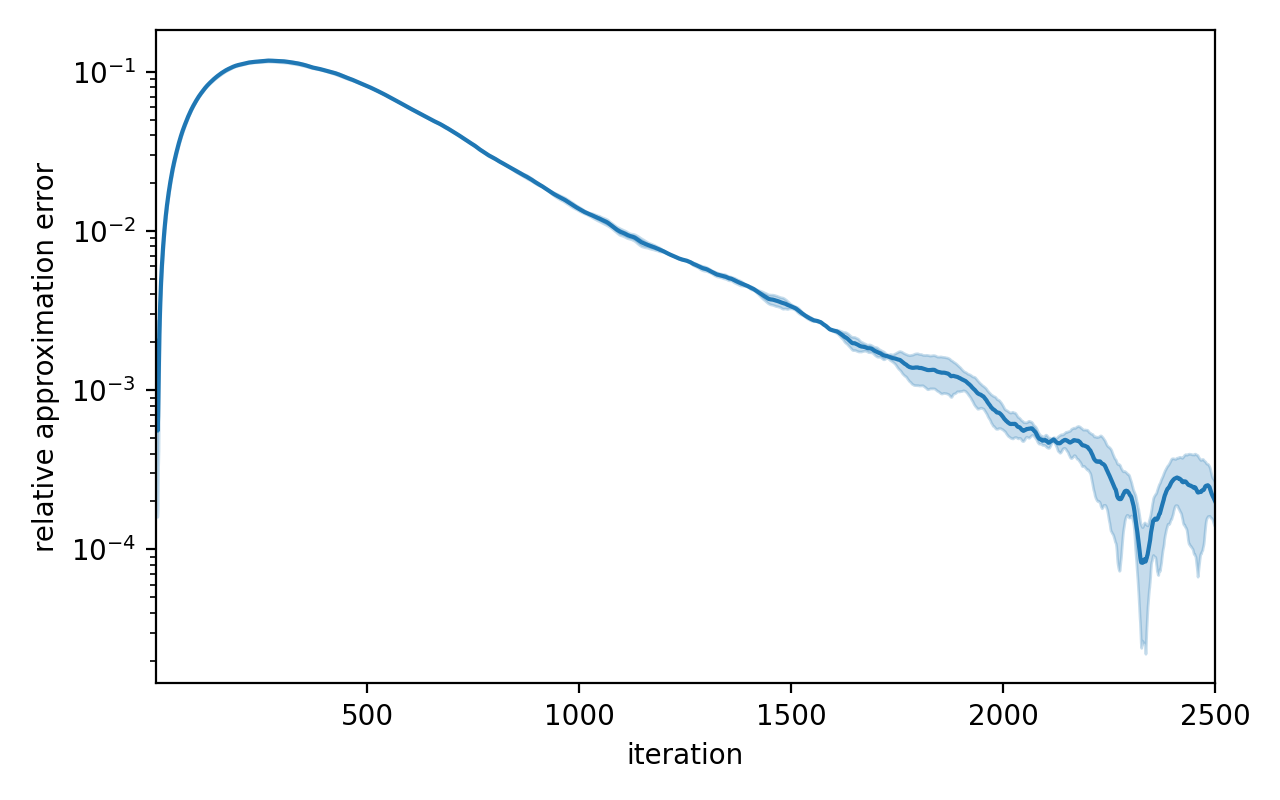
\includegraphics[width=0.48\linewidth]{figures/deep_bsde_pnas_hjb_error.png}\hfill
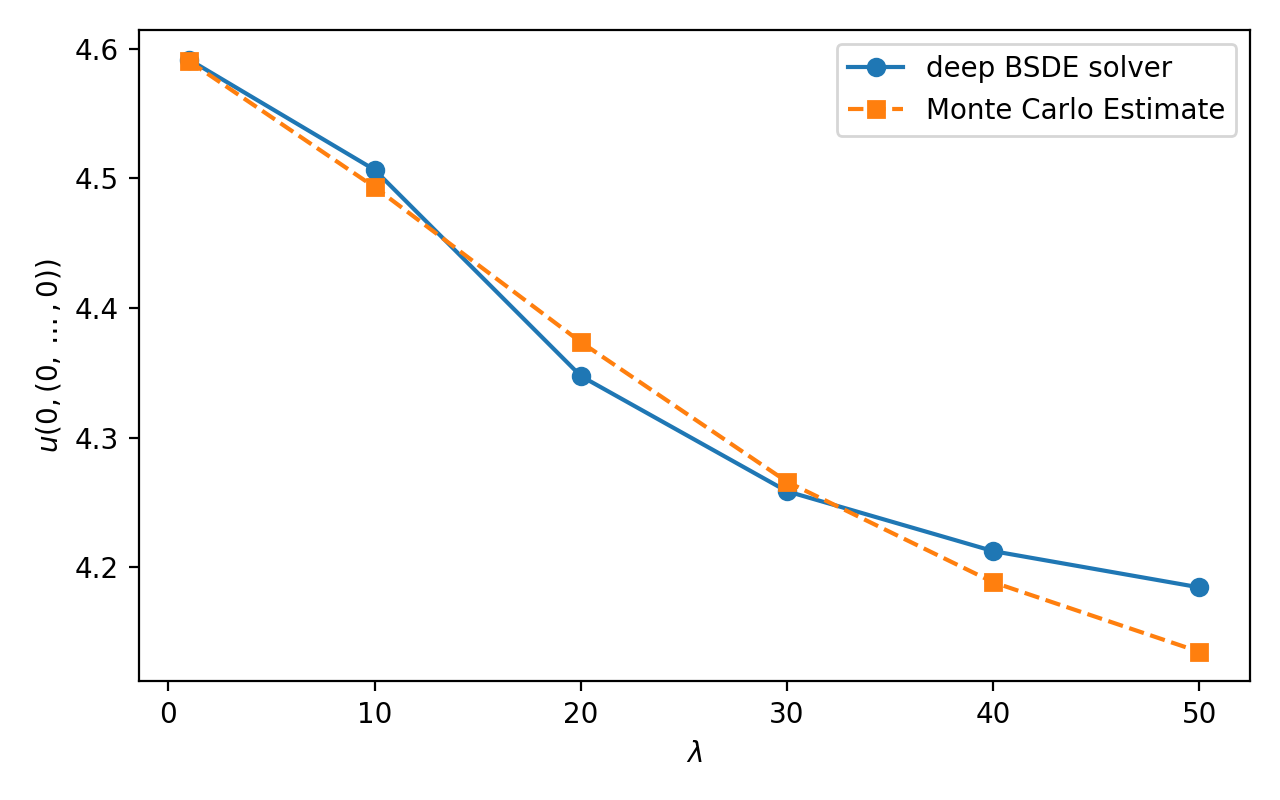
\includegraphics[width=0.48\linewidth]{figures/deep_bsde_pnas_hjb_lambda.png}
\caption{Relative error at $\lambda = 1$ (left) and $u(0,(0,\ldots,0))$ for  $\lambda \in \{1,10,20,30,40,50\}$, compare Fig.~2 of \cite{Han2018}.}
\label{fig:hjb}
\end{figure}

\subsection{Allen-Cahn Equation}
\label{sec:ac}
We analyze an Allen-Cahn equation in $100$ dimensions, given by the initial value problem
\begin{equation}
\partial_t u(t,x) = \Delta u(t,x) + u(t,x) - u(t,x)^3,
\qquad
u(0,x) = g(x) = \frac{1}{2 + 0.4\,\lVert x\rVert^2}.
\label{eq:ac}
\end{equation}
No closed-form solution is available. The comparison value
\begin{equation}
u(0.3,(0,\dots,0)) \approx 0.0528
\end{equation}
was computed with the branching-diffusion method in the paper. The deep BSDE method expects a semilinear parabolic terminal value problem, so we reverse time. We set
\begin{equation}
v(t,x) := u(T-t,\,x), \qquad (t,x)\in[0,T]\times\mathbb R^{100},
\end{equation}
and compute, by the chain rule,
\begin{align}
\partial_t v(t,x) &= -\left(\partial_t u\right)(T-t,x),
\nonumber\\
\Delta v(t,x) &= (\Delta u)(T-t,x),
\nonumber\\
v(T,x) &= u(0,x) = g(x).
\end{align}
Evaluating \eqref{eq:ac} at the time point $T-t$ and substituting gives
\begin{align*}
-\partial_t v(t,x) &= \Delta v(t,x) + v(t,x) - v(t,x)^3,
\\
0 &= \partial_t v(t,x) + \Delta v(t,x) + v(t,x) - v(t,x)^3,
\qquad
v(T,x) = g(x),
\end{align*}
which is the desired form. The corresponding forward-backward system reads
\begin{align}
X_t &= \sqrt2\,W_t, \nonumber\\
\mathrm dY_t &= -\left(Y_t - Y_t^3\right)\mathrm dt
+ Z_t^{\top}\mathrm dW_t,
\qquad Y_T = g(X_T),
\label{eq:ac-fbsde}
\end{align}
with
\begin{equation}
Y_t = v(t,X_t),
\qquad
Z_t = \sqrt2\,\nabla v(t,X_t).
\end{equation}
The deep BSDE solver applied to \eqref{eq:ac-fbsde} approximates
\begin{equation}
v(0,0) = u(T,(0,\dots,0)),
\end{equation}
so training with horizon $T$ returns the value of the original solution
at time $T$. We specified the parameters according to Table~\ref{tab:ac-params}.
\begin{table}[htb]
\centering
\begin{tabular}{llll}
\toprule
$d$ & $100$ & time steps $N$ & $20$ \\
$T$ & $0.3$ & learning rate & $10^{-3}$, decaying to $10^{-4}$ \\
$x$ & $(0,\dots,0)$ & iterations & $4000$\\
& & batch size & $64$\\
\bottomrule
\end{tabular}
\caption{Parameters of the Allen-Cahn example.}
\label{tab:ac-params}
\end{table}
Figure~\ref{fig:ac} (left) shows the relative error of $\hat u_{\mathrm{NN}}$ at $t=0.3$ against the number of iteration steps. We obtain
\begin{equation}
\hat u_{\mathrm{NN}} = \acYzero,
\qquad
\frac{\left|\hat u_{\mathrm{NN}} - 0.0528\right|}{0.0528}
= \acRelErr\,\%,
\end{equation}
against $0.30\,\%$ in the paper. Figure~\ref{fig:ac} (right) shows the
time evolution of $u(t,(0,\dots,0))$, obtained by repeating the training for the times $t \in\{0.02, 0.05, 0.08, 0.11, 0.14, 0.18, 0.22, 0.26, 0.30\}$.
\begin{figure}[htb]
\centering
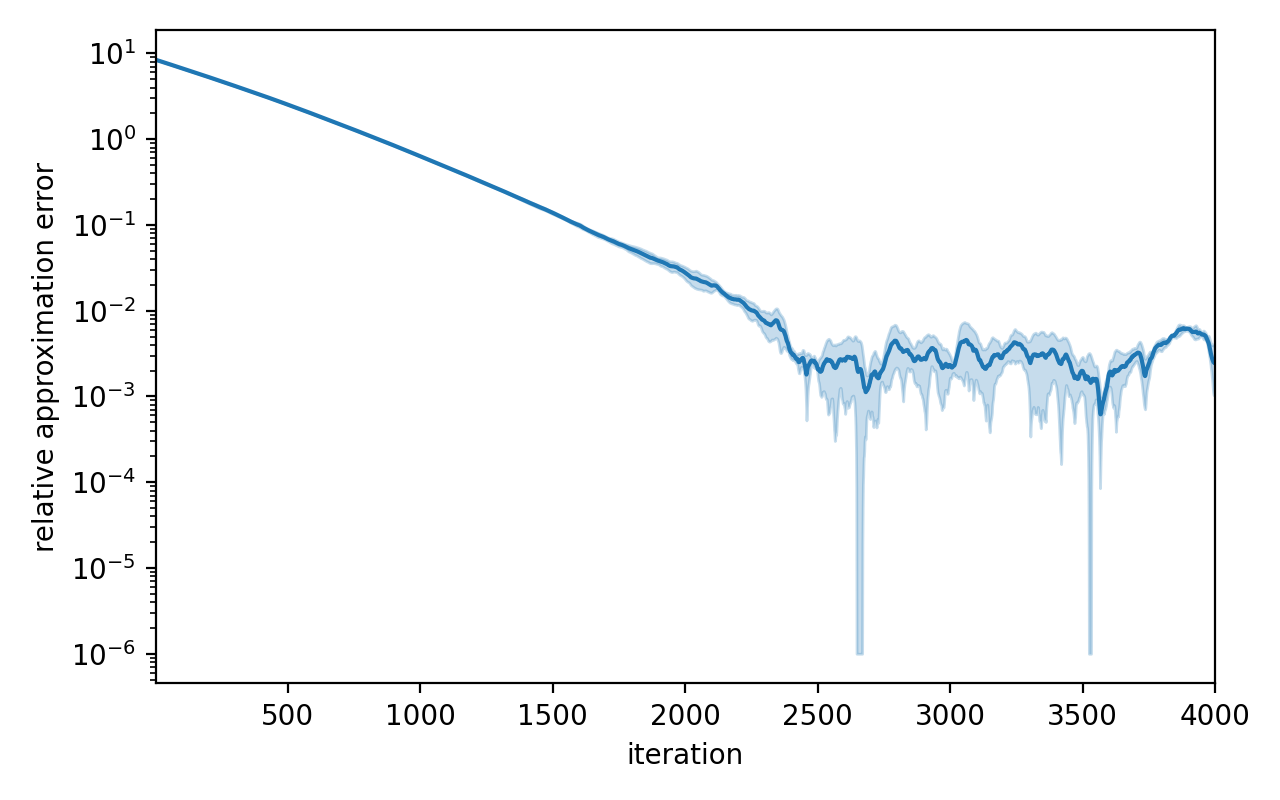
\includegraphics[width=0.48\linewidth]{figures/deep_bsde_pnas_allencahn_error.png}\hfill
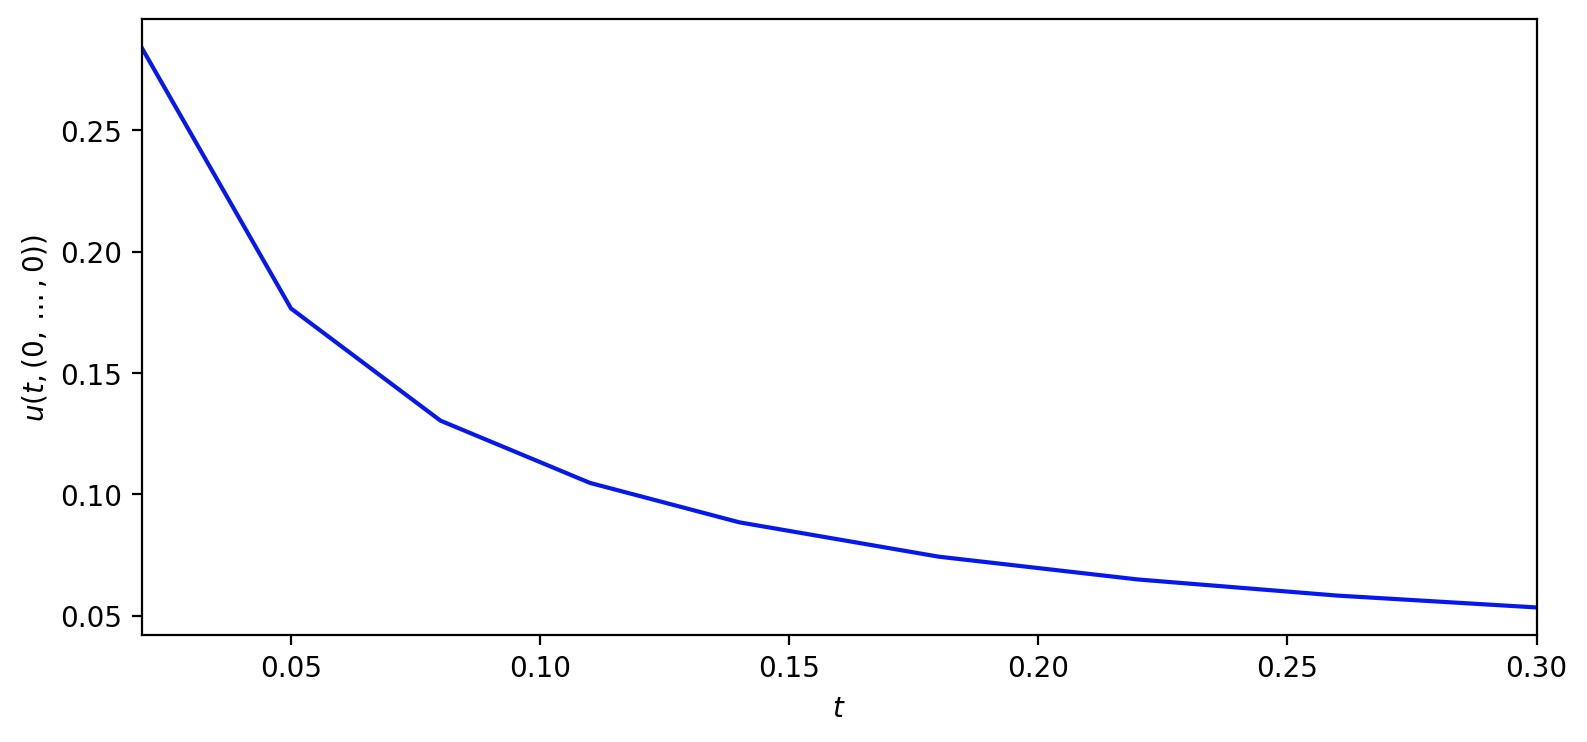
\includegraphics[width=0.48\linewidth]{figures/deep_bsde_pnas_allencahn_time.png}
\caption{Allen-Cahn equation, relative error at $T = 0.3$ (left) and time
evolution of $u(t,(0,\dots,0))$ (right), compare Fig.~3 of
\cite{Han2018}.}
\label{fig:ac}
\end{figure}
\subsection{Nonlinear Black-Scholes Equation with Default Risk}
\label{sec:dr}
We start from the classical Black-Scholes equation. For a single underlying with volatility $\bar\sigma$ and risk-free rate $r$, the arbitrage-free price $u(t,x)$ of a European derivative with payoff $g$ solves the linear terminal value problem
\begin{equation}
\partial_t u(t,x) + r\,x\,\partial_x u(t,x)
+ \frac{\bar\sigma^2}{2}\,x^2\,\partial_{xx}^2 u(t,x) - r\,u(t,x) = 0,
\qquad
u(T,x) = g(x),
\label{eq:bs-classical}
\end{equation}
where $x$ is the current price of the underlying. The paper augments \eqref{eq:bs-classical} in two directions. First, the claim depends on $100$ underlyings following componentwise geometric Brownian motion,
\begin{equation*}
\mathrm dX_t^{i} = \bar\mu\, X_t^{i}\,\mathrm dt
+ \bar\sigma\, X_t^{i}\,\mathrm dW_t^{i},
\qquad i = 1,\dots,100,
\end{equation*}
and pays the minimum of the underlyings at maturity,
\begin{equation*}
g(x) = \min(x_1,\dots,x_{100}).
\end{equation*}
Second, the issuer may default. Default is modeled as the first jump of a
Poisson process whose intensity $Q(u)$ is a decreasing function of the
current value $u$, default becomes more likely when the claim is worth
less. The intensity is piecewise linear with three regions,
\begin{equation}
Q(y) = \mathbf 1_{(-\infty,v^h)}(y)\,\gamma^h
+ \mathbf 1_{[v^l,\infty)}(y)\,\gamma^l
+ \mathbf 1_{[v^h,v^l)}(y)
  \left[\frac{\gamma^h-\gamma^l}{v^h-v^l}\left(y-v^h\right)+\gamma^h\right].
\label{eq:dr-intensity}
\end{equation}
\begin{figure}[htb]
\centering
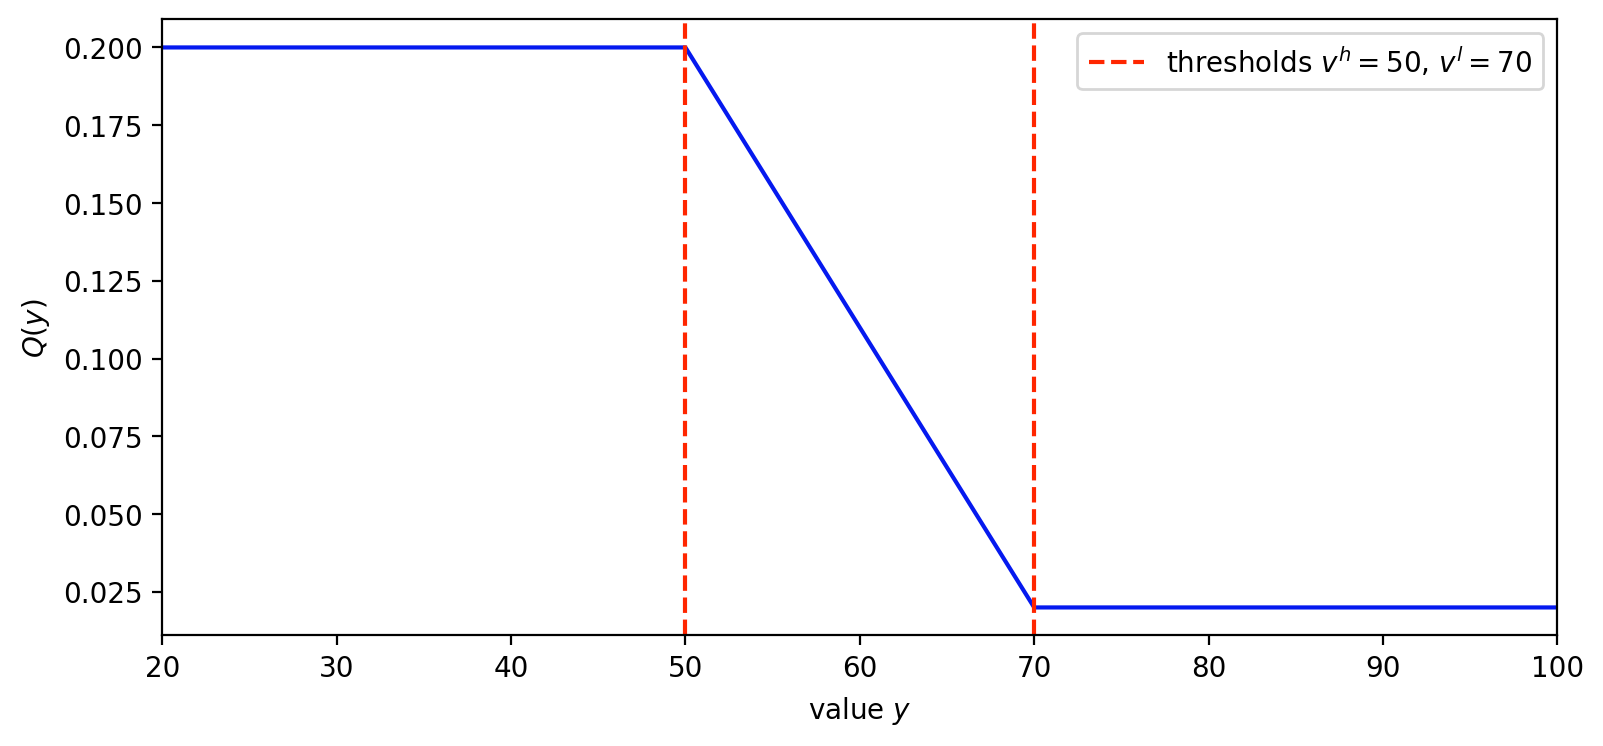
\includegraphics[width=0.62\linewidth]{figures/deep_bsde_pnas_default_intensity.png}
\caption{The default intensity $Q$ of \eqref{eq:dr-intensity}.}
\label{fig:dr-intensity}
\end{figure}
The three parts of \eqref{eq:dr-intensity} correspond to three value
regimes. If the current value $y$ lies below the lower threshold $v^h$,
the default intensity takes the high constant level $\gamma^h$, a claim
with high default probability. If $y$ lies above the upper threshold
$v^l$, the intensity takes the low constant level $\gamma^l$, so the default probability is low. Between the thresholds the $Q$ is linearly interpolated between the two levels. Figure~\ref{fig:dr-intensity} shows its graph. The parameters $\gamma^h$ and $\gamma^l$ are therefore the default intensities in the high and low risk regimes. At default the holder recovers only the fraction $\delta \in [0,1)$ of the current value. The default rate enters the equation via the term
\begin{equation}
\left(1-\delta\right) Q\!\left(u\right) u,
\end{equation}
additionally with a discounting component $Ru$. The extended PDE takes the form
\begin{equation*}
\partial_t u
+ \bar\mu\, x \cdot \nabla u
+ \frac{\bar\sigma^2}{2} \sum_{i=1}^{100} \lvert x_i\rvert^2\,
  \frac{\partial^2 u}{\partial x_i^2}
- \left(1-\delta\right) Q\!\left(u\right) u - R\, u = 0,
\qquad
u(T,x) = g(x),
\end{equation*}
which is a semilinear parabolic terminal value problem with
\begin{equation*}
\mu(x) = \bar\mu\,x,
\qquad
\sigma(x) = \bar\sigma\operatorname{diag}(x),
\qquad
f(t,x,y,z) = -\left(1-\delta\right)Q(y)\,y - R\,y.
\end{equation*}
Here, again no closed-form solution is available. The comparison value
\begin{equation}
u(0,(100,\dots,100)) \approx 57.300
\end{equation}
was computed with the multilevel Picard method \cite{EHJK2019}, as quoted in the paper.
\begin{figure}[htb]
\centering
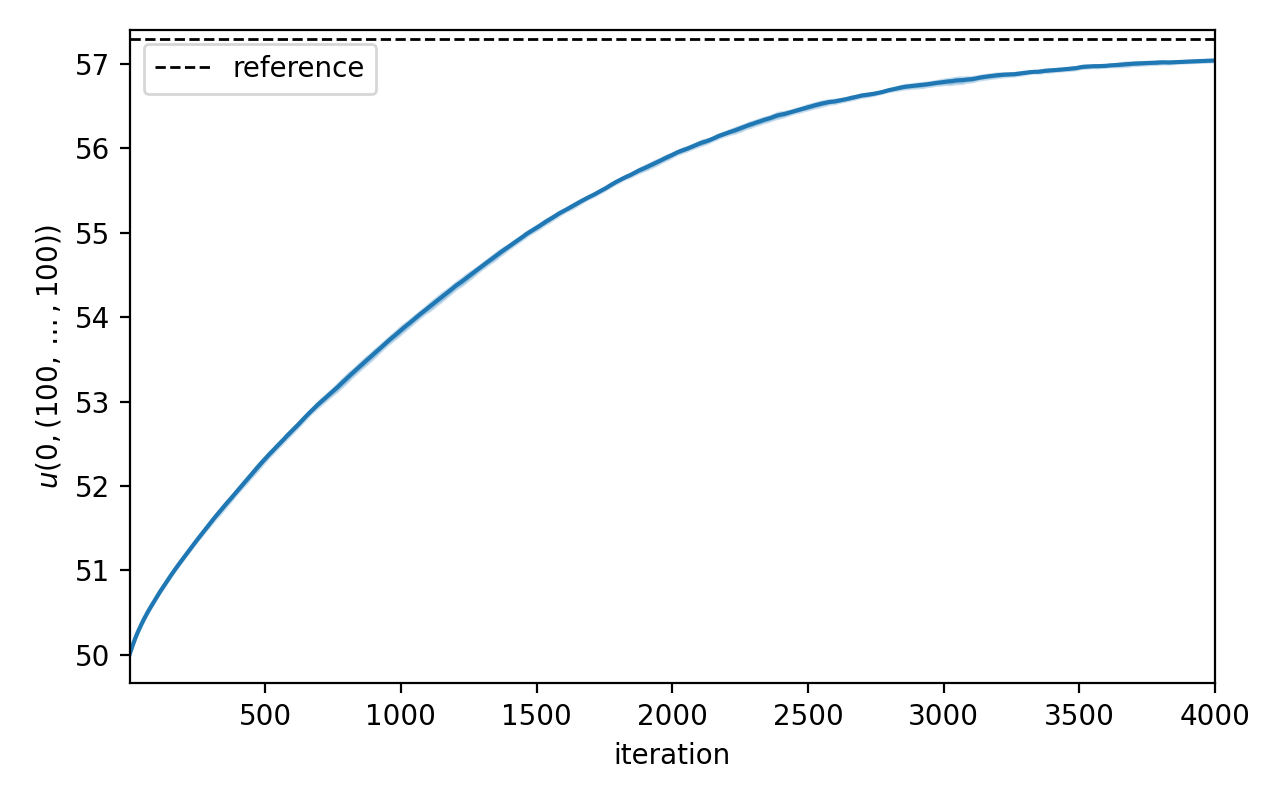
\includegraphics[width=0.62\linewidth]{figures/deep_bsde_pnas_default_risk_y0.png}
\caption{Default risk, approximation of $u(0,(100,\dots,100))$, compare
Fig.~1 of \cite{Han2018}.}
\label{fig:dr}
\end{figure}
The backward equation in this case reads
\begin{align*}
\mathrm dY_t &= \left[\left(1-\delta\right)Q\!\left(Y_t\right) + R\right]
Y_t\,\mathrm dt + Z_t^{\top}\mathrm dW_t,
\qquad Y_T = \min\!\left(X_T^1,\dots,X_T^{100}\right),
\end{align*}
with
\begin{equation}
Y_t = u(t,X_t),
\qquad
Z_t = \bar\sigma\operatorname{diag}(X_t)\,\nabla u(t,X_t)
\end{equation}
with parameters in Table~\ref{tab:dr-params}.
\begin{table}[htb]
\centering
\begin{tabular}{llllll}
\toprule
$d$ & $100$ & $\delta$ & $2/3$ & time steps $N$ & $40$ \\
$T$ & $1$ & $R$ & $0.02$ & learning rate & $10^{-2}$, decaying to $10^{-3}$ \\
$\bar\mu$ & $0.02$ & $v^h,\,v^l$ & $50,\,70$ & iterations & $4000$ \\
$\bar\sigma$ & $0.2$ & $\gamma^h,\,\gamma^l$ & $0.2,\,0.02$ & batch size & $64$ \\
$X_0$ & $(100,\dots,100)$ & start of $\theta_{u_0}$ & $50$ & & \\
\bottomrule
\end{tabular}
\caption{Parameters of the default-risk example.}
\label{tab:dr-params}
\end{table}
Figure~\ref{fig:dr} shows the approximation of $u(0,(100,\dots,100))$
against the number of iteration steps. We obtain an estimate and error of
\begin{equation}
\hat u_{\mathrm{NN}} = \drYzero,
\qquad
\frac{\left|\hat u_{\mathrm{NN}} - 57.300\right|}{57.300}
= \drRelErr\,\%,
\end{equation}
against $0.46\,\%$ in the paper.


\subsection{Reaction-Diffusion Equation}
\label{sec:rd}
The last example of the paper is the time-dependent reaction-diffusion equation
\begin{equation}
\partial_t u(t,x) + \tfrac12\,\Delta u(t,x)
+ \min\!\left\{1,\left(u(t,x) - u^{*}(t,x)\right)^2\right\} = 0,
\qquad
u(T,x) = u^{*}(T,x),
\label{eq:rd}
\end{equation}
with the function
\begin{equation*}
u^{*}(t,x) = 1 + \kappa
+ \sin\!\Big(\lambda\sum_{i=1}^{d} x_i\Big)
\exp\!\left(\frac{\lambda^2 d\,(t-T)}{2}\right),
\qquad
\kappa = 0.6,
\quad
\lambda = \tfrac{1}{\sqrt d}.
\end{equation*}
The function $u^{*}$ itself solves \eqref{eq:rd}. Writing $s(x) := \sin\!\big(\lambda\sum_i x_i\big)$ and
$e(t) := \exp\!\big(\lambda^2 d\,(t-T)/2\big)$ we compute
\begin{align}
\partial_t u^{*}(t,x) &= \frac{\lambda^2 d}{2}\, s(x)\, e(t),
\nonumber\\
\Delta u^{*}(t,x) &= -\lambda^2 d\, s(x)\, e(t),
\end{align}
so $\partial_t u^{*} + \tfrac12\Delta u^{*} = 0$, the reaction term vanishes at $u = u^{*}$, and the terminal condition holds by construction. The exact value at the origin is
\begin{equation}
u(0,(0,\dots,0)) = 1 + \kappa = 1.6 .
\end{equation}
Equation \eqref{eq:rd} is a semilinear parabolic terminal value problem with
\begin{equation}
\mu = 0,
\qquad
\sigma = I_d,
\qquad
f(t,x,y,z) = \min\!\left\{1,\left(y - u^{*}(t,x)\right)^2\right\}.
\end{equation}
In the paper, it got solved with $0$ to $4$ hidden layers per subnetwork and $40000$ iterations and reports that the relative error
decreases in the number of hidden layers. We reconstruct the study for
$1$ to $4$ hidden layers at the 40000 epochs of training of the paper. We specified the parameters according to Table~\ref{tab:rd-params}. Since
the terminal condition at $t=0$ already is the exact value, we
start $\theta_{u_0}$ away from the solution at $0.5$.

\begin{table}[htb]
\centering
\begin{tabular}{llll}
\toprule
$d$ & $100$ & time steps $N$ & $30$ \\
$T$ & $1$ & learning rate & $10^{-2}$, decaying to $3\cdot10^{-4}$ \\
$\kappa$ & $0.6$ & subnetwork rate factor & $0.1$ \\
$\lambda$ & $0.1$ & iterations & $40000$ \\
$x$ & $(0,\dots,0)$ & batch size & $64$ \\
hidden layers & $1, 2, 3, 4$ & start of $\theta_{u_0}$ & $0.5$ \\
\bottomrule
\end{tabular}
\caption{Parameters of the reaction-diffusion example.}
\label{tab:rd-params}
\end{table}
Table~\ref{tab:rd-results} and Figure~\ref{fig:rd} compare the relative
errors per network depth with Table~1 of the paper, at the $40000$
iterations of the paper. The error decreases in the number of hidden
layers. At four hidden layers it reaches $0.93\,\%$ against
$0.53\,\%$ in the paper, the first two depths end on the same level
near $2.5\,\%$, and only the deeper networks push below it.
\begin{table}[htb]
\centering
\begin{tabular}{lcccc}
\toprule
hidden layers & $1$ & $2$ & $3$ & $4$ \\
\midrule
this reconstruction
  & $2.49\,\%$ & $2.48\,\%$ & $1.72\,\%$ & $0.93\,\%$ \\
paper
  & $0.90\,\%$ & $0.60\,\%$ & $0.56\,\%$ & $0.53\,\%$ \\
\bottomrule
\end{tabular}
\caption{Relative error per number of hidden layers.}
\label{tab:rd-results}
\end{table}

\begin{figure}[htb]
\centering
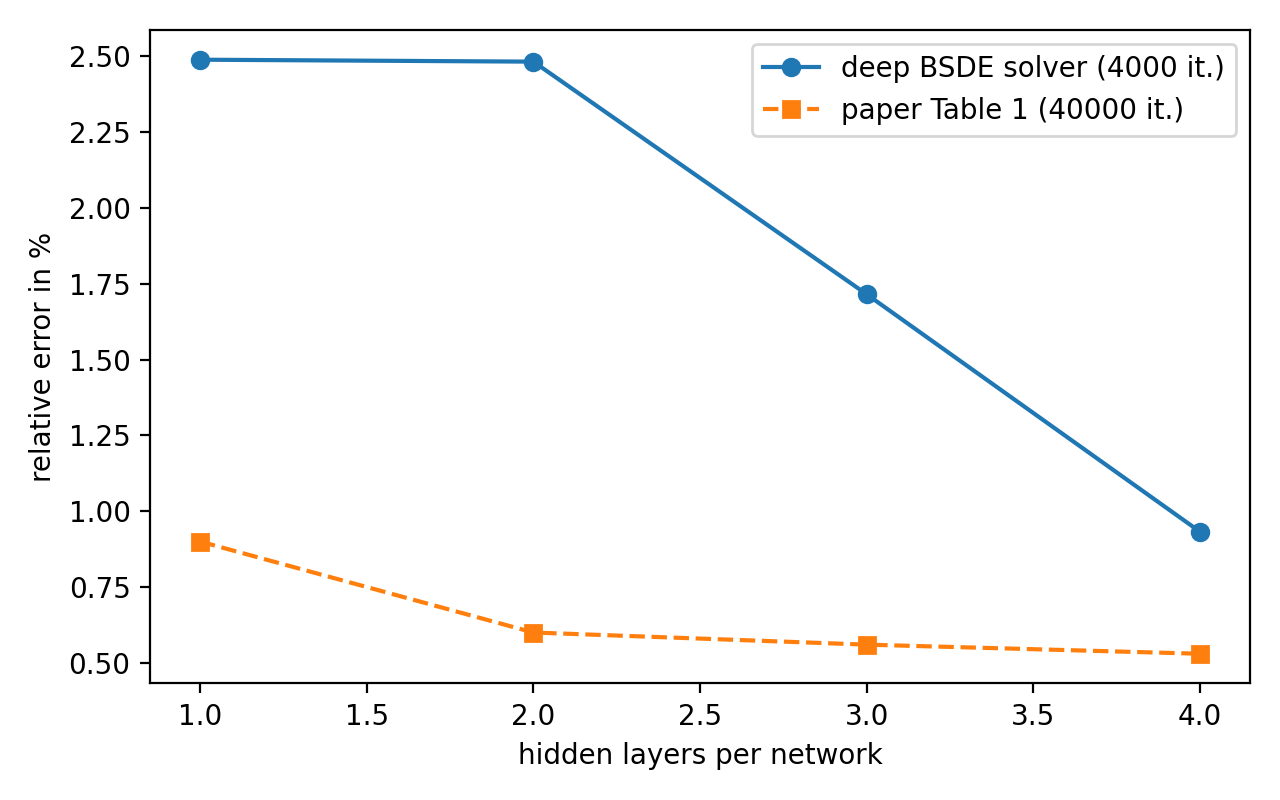
\includegraphics[width=0.62\linewidth]{figures/deep_bsde_pnas_layers.png}
\caption{Relative error against the number of hidden layers, compare
Table~1 of \cite{Han2018}.}
\label{fig:rd}
\end{figure}

\subsection{Stability in the Starting Value}
\label{sec:init-stability}

Each example is trained again from four starting values of the
trainable initial value $\widehat Y_0$, one seed per value and all
other settings unchanged. Figure~\ref{fig:init-stability} collects the
four runs, panel (a) shows the HJB equation, (b) the Allen-Cahn
equation, (c) the default risk equation and (d) the
reaction-diffusion equation. Every
curve moves toward the reference, and no run diverges or settles at a
wrong level. The further away the start is, the more iterations the
curve needs to get there. The starts furthest away in the first two
equations have not fully arrived after $5000$ iterations, while in the
default risk example $10000$ iterations bring even the starts of $20$
and $90$ close to the reference, although they begin deep in the high
and low risk regime of $Q$. The reaction-diffusion runs collapse onto a common
path within a few hundred iterations and settle together slightly
above the benchmark, so the remaining error stems from the method and
not from the initialization.

\begin{figure}[htb]
\centering
\begin{subfigure}{0.48\linewidth}\centering
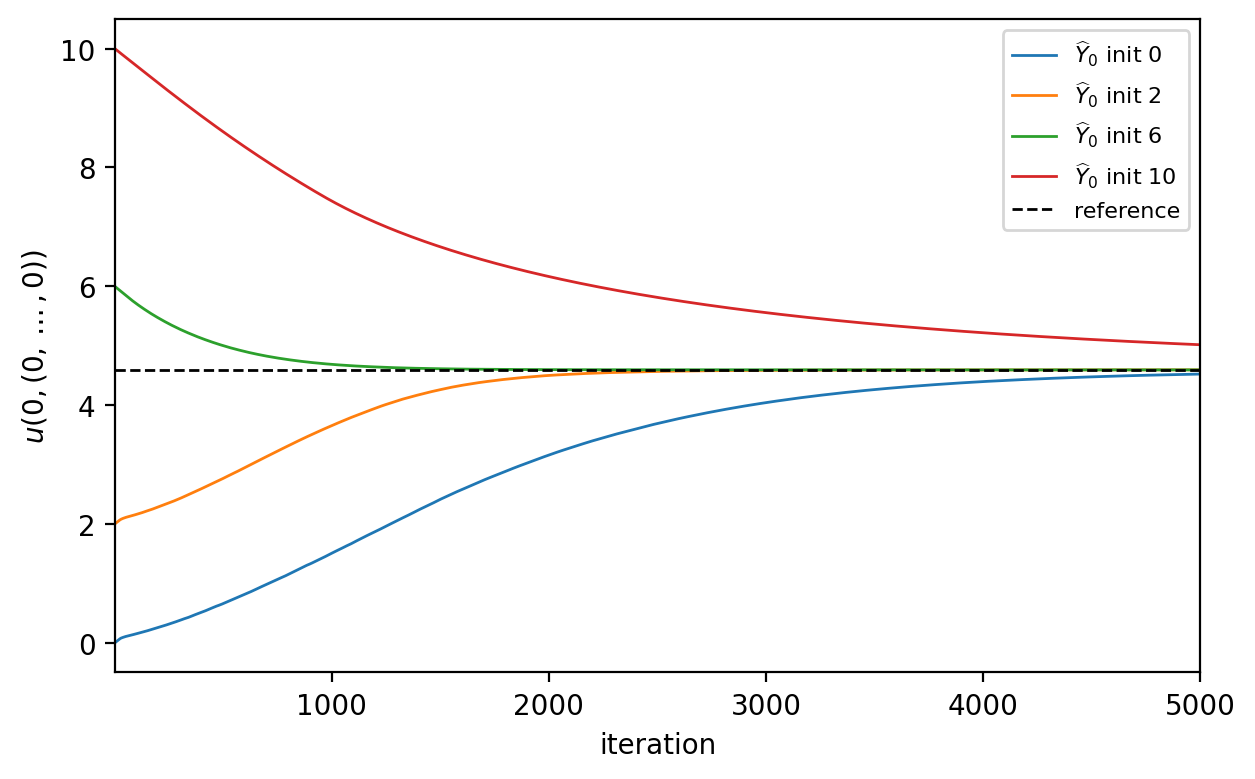
\includegraphics[width=\linewidth]{figures/deep_bsde_pnas_hjb_init_stability.png}
\caption{Hamilton-Jacobi-Bellman}
\end{subfigure}\hfill
\begin{subfigure}{0.48\linewidth}\centering
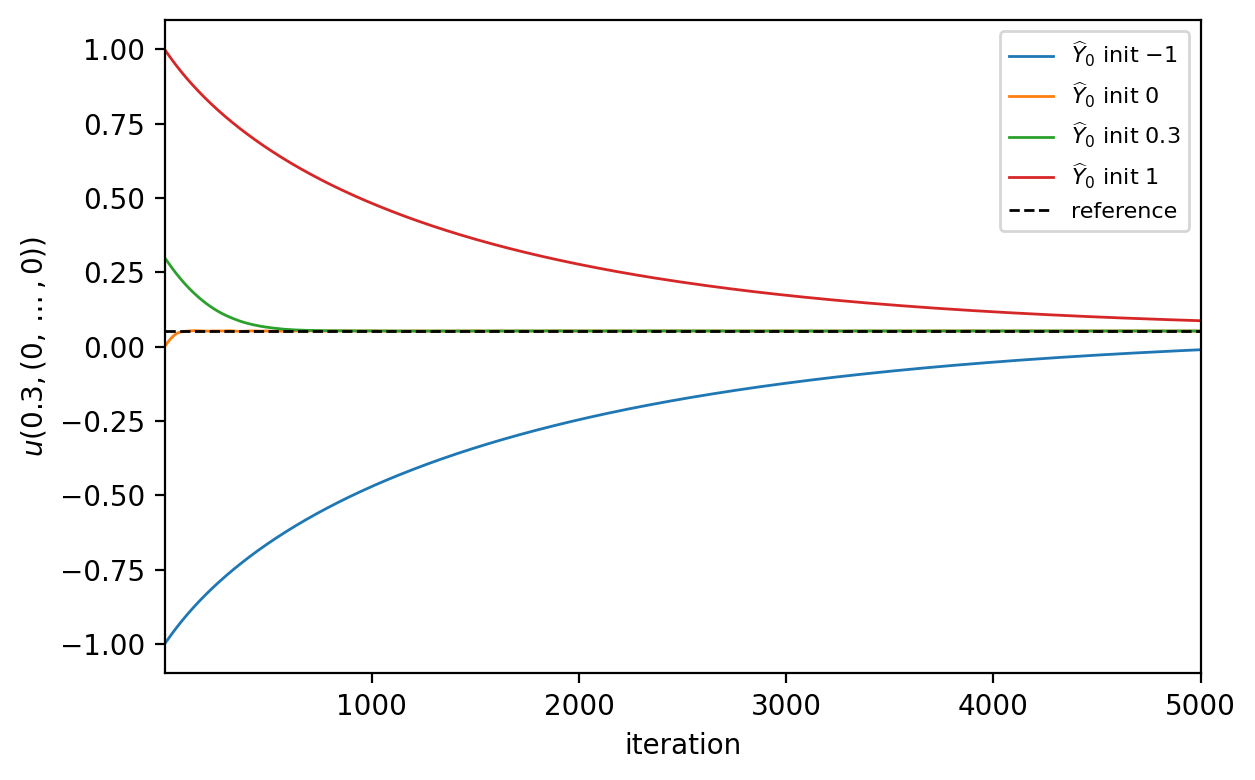
\includegraphics[width=\linewidth]{figures/deep_bsde_pnas_allencahn_init_stability.png}
\caption{Allen-Cahn}
\end{subfigure}\\[0.3em]
\begin{subfigure}{0.48\linewidth}\centering
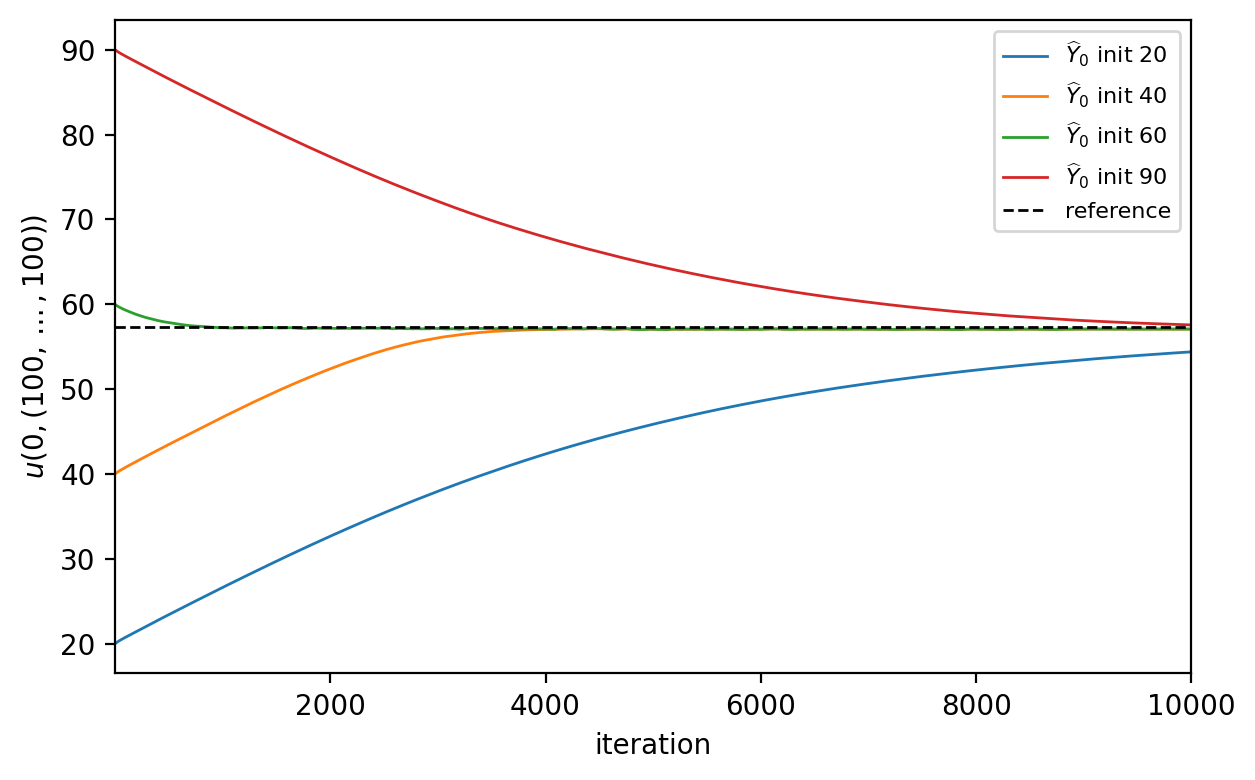
\includegraphics[width=\linewidth]{figures/deep_bsde_pnas_default_risk_init_stability.png}
\caption{default risk}
\end{subfigure}\hfill
\begin{subfigure}{0.48\linewidth}\centering
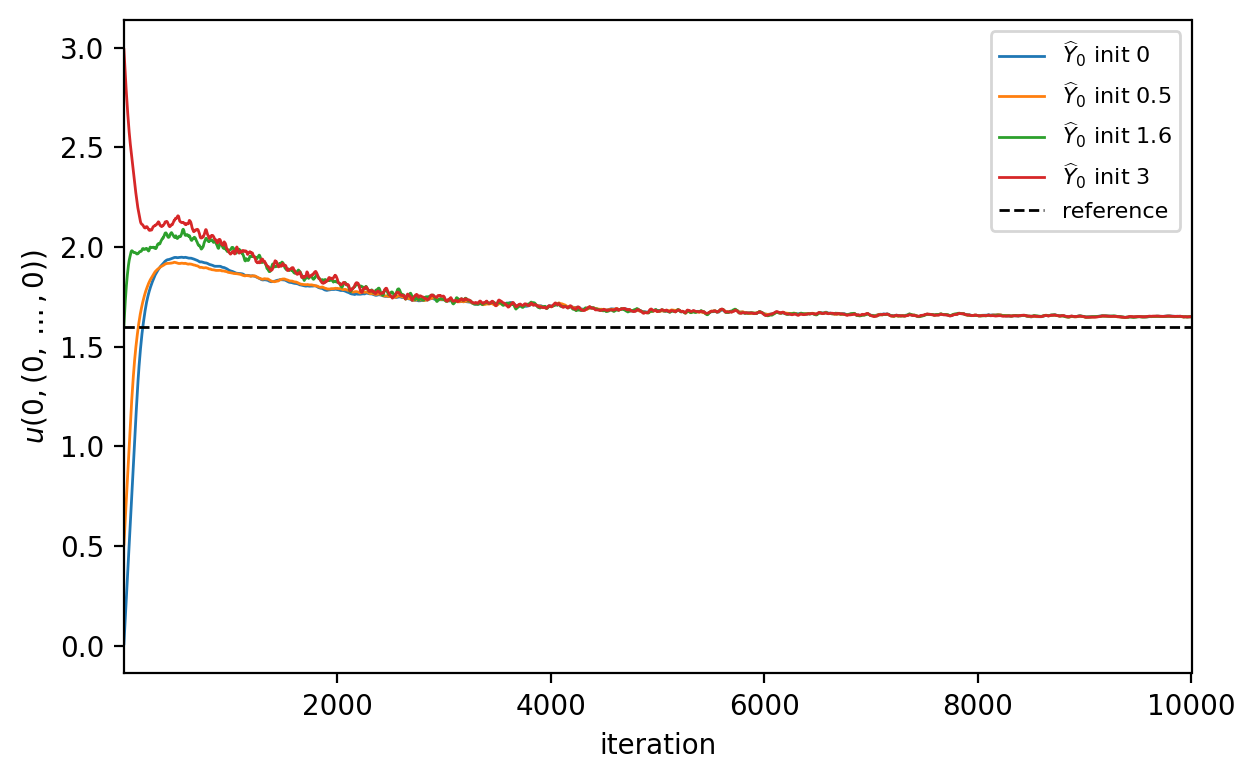
\includegraphics[width=\linewidth]{figures/deep_bsde_pnas_reaction_diffusion_init_stability.png}
\caption{reaction-diffusion}
\end{subfigure}
\caption{Training from four starting values of $\widehat Y_0$ per
example.}
\label{fig:init-stability}
\end{figure}

\section{Conclusion}
\label{sec:conclusion}
We could replicate all four examples of \cite{Han2018}. The errors match the accuracy reported in the paper, and the hidden-layer study reproduces the trend of the paper's Table~1 and comes close to its level. All runs together take a few hours on a laptop CPU. We have made the following observations.
\begin{itemize}
    \item [(1)] The choice of the starting value can have an effect on how long effective training takes, but the optimization was successful for all tested initializations, see Section~\ref{sec:init-stability}.
    \item [(2)] The accuracy of the examples could often be reached, sometimes even improved.
    \item [(3)] The $100$-dimensional examples do not need substantially more time than lower dimensional ones, so we have verified that the curse of dimensionality can indeed be overcome by this method.
\end{itemize}


\begin{thebibliography}{9}
\bibitem{Han2018}
J.~Han, A.~Jentzen, W.~E,
\emph{Solving high-dimensional partial differential equations using deep
learning}, Proceedings of the National Academy of Sciences 115(34),
8505--8510, 2018.

\bibitem{DeepBSDErepo}
J.~Han,
\emph{DeepBSDE, Deep BSDE solver in TensorFlow},
\url{https://github.com/frankhan91/DeepBSDE}.

\bibitem{PardouxPeng1990}
E.~Pardoux, S.~Peng,
\emph{Adapted solution of a backward stochastic differential equation},
Systems \& Control Letters 14(1), 55--61, 1990.

\bibitem{ElKarouiPengQuenez1997}
N.~El~Karoui, S.~Peng, M.~C.~Quenez,
\emph{Backward stochastic differential equations in finance},
Mathematical Finance 7(1), 1--71, 1997.

\bibitem{Oksendal2003}
B.~{\O}ksendal,
\emph{Stochastic Differential Equations, An Introduction with
Applications}, 6th edition, Springer, Berlin, 2003.

\bibitem{EHJK2019}
W.~E, M.~Hutzenthaler, A.~Jentzen, T.~Kruse,
\emph{On multilevel Picard numerical approximations for high-dimensional
nonlinear parabolic partial differential equations and high-dimensional
nonlinear backward stochastic differential equations},
Journal of Scientific Computing 79(3), 1534--1571, 2019.
\end{thebibliography}

\listoffigures

\end{document}
